
\documentclass[a4paper,12pt,oneside]{report}

\usepackage{colortbl}

\usepackage{phdthesis}

\usepackage{kostspielig}

\usepackage{pifont}

\newcommand{\todo}[1]{\textcolor{red}{\textbf{TODO: #1}}}


\title{Design Iteration 4}
\subtitle{Open-source web-app for questionnaires and surveys}
\date{Winter 2011}
\location{University of California Irvine}
\author{Kevin Brotcke\\
Maria Carrasco\\
Andrew Furusawa\\\
Joshua Papa }

\begin{document}
   
\renewcommand{\contentsname}{Contents}
\renewcommand{\bibname}{Bibliography}
\renewcommand{\caption}{{\bf Caption : }}

\raskolnikovmaketitle
\tableofcontents

\chapter{Introduction}

\section{ Purpose}

This document describes the design layout for the Survey Generator program by Team 1000 for their Informatics 117 class during Winter 2011. Major design components such as the data design, architectural and component-level design, and user interface design will be discussed. This is meant as a reference for team members during implementation as well evidence for stakeholders.
\section{ Project Description}

        The project uses a database back-end to generate surveys on-the-fly using a web app. The main components consists of a SQLite database, HTML front-end of surveys and administrator panel, and business logic to generate the surveys.
\chapter{ Data Design}
\section{ Database Description}

        The data will be stored in the form of an embedded SQLite database. (See figure \ref{database})
\section{ Temporary Data Structures}

This will need to import and export XML files in the form XLSX as well as CSV files. These will
only be temporary since they are being converted into and out of the SQLite database.
\chapter{Design Pattern : MVC}
For our application we decided to use the \emph{Model View Controller} pattern. This decision was made based on the fact that this pattern is the most used for today's world web applications.
\vskip 1cm
\begin{figure}[h!]
  \begin{center}
   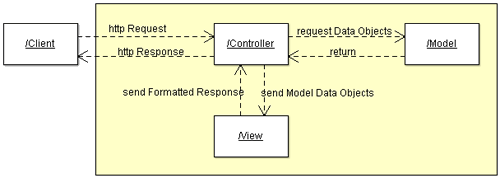
\includegraphics[width=10.5cm]{pics/mvc1.png}
  \end{center}
\caption{MVC Collaboration Diagram.}
\end{figure}

\vskip 1.5cm
The \emph{MVC} pattern divides our application in three main modules:\\
\begin{description}
\item[Model]  \ding{32} \\ \\
This module is responsible for managing the data. It is responsible for storing and retrieving information from the database, in our case \emph{SQLite}. \\
\item[View]  \ding{32} \\ \\
The view is the module that display the data provided by the model in a specific format. \\
\item[Controller]  \ding{32}  \\ \\
The controller is responsible to handle the other two models working together. This module receives a request from a client, invokes the \emph{model} to perform the requested operations and send the resulting data to the \emph{view}. The view is in charged to  format the resulting data to be presented to the user. This format is in HTML format.
\end{description}

\chapter{ Architectural and Component-level Design}
\section{ System Structure}
\subsection{ Architecture Diagram}
\begin{figure}[h!]
  \begin{center}
   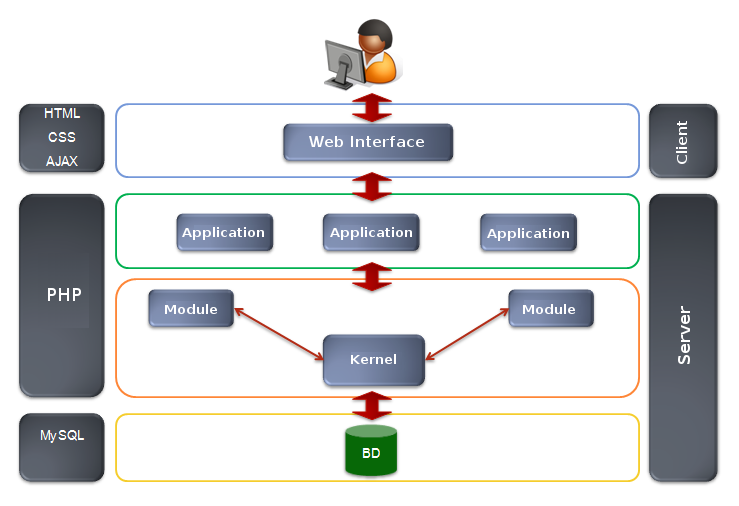
\includegraphics[width=13.7cm]{pics/ar.png}
  \end{center}
\caption{Block Diagram showing major components.}
\end{figure}

The figure shows the \emph{Architectural Diagram}. This diagram shows the main components in our application. The main characteristic the application will be divided in different levels of interaction. 

The database will only interact with the \emph{Modules}, that will be responsible for retrieving and storing data from the database.

 The \emph{Application} will be responsible for controlling the interaction between the user and the database. Through the \emph{Web Interface} the user will request information that the application will receive invoking the correct module.

The tools used to develop the System are HTML, CSS, PHP and SQLite.

\newpage

\section{Class Diagram}
\vskip 2cm
\label{database}
\begin{figure}[h!]
  \begin{center}
   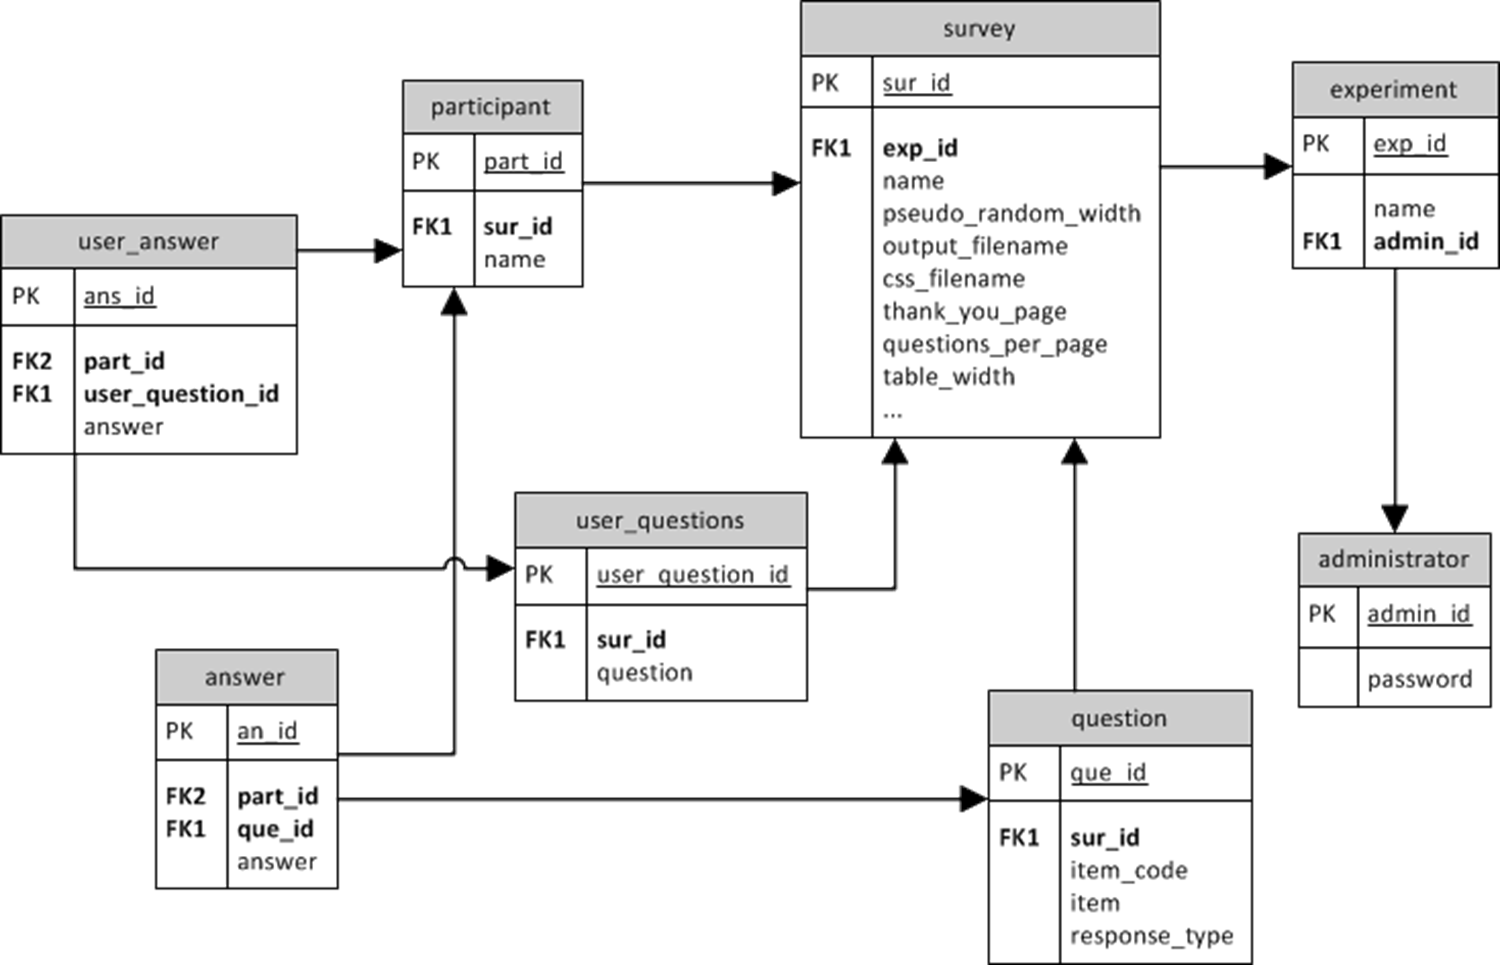
\includegraphics[width=15.5cm]{pics/class.png}
  \end{center}
\caption{Class Diagram.}
\end{figure}

\newpage

\section{Sequence Diagrams}
\vskip 1 cm
These interaction diagrams show the order of operation of the different processes or objects in our system. The interact with each other by sending messages (represented by the horizontal arrows).
\vskip 2.5cm
\subsection{Request Survey}
\vskip 1.5cm
\begin{figure}[!hp]
  \begin{center}
   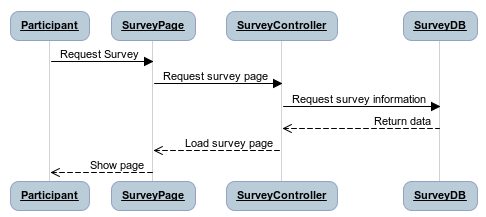
\includegraphics[width=11cm]{pics/request.png}
  \end{center}
\caption{Request Suvey Sequence Diagram.}
\end{figure}
\newpage
\subsection{Submit Survey}
%\vskip 1cm
\begin{figure}[!hp]
  \begin{center}
   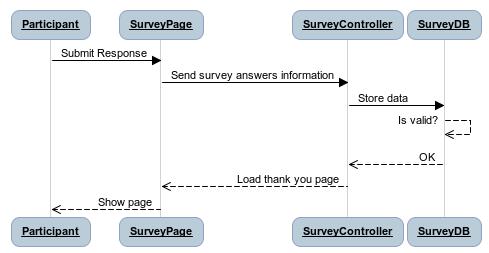
\includegraphics[width=10.5cm]{pics/submit.png}
  \end{center}
\caption{Submit Survey Sequence Diagram.}
\end{figure}
\vskip 2cm
\subsection{Login}
%\vskip 1cm
\begin{figure}[!hp]
  \begin{center}
   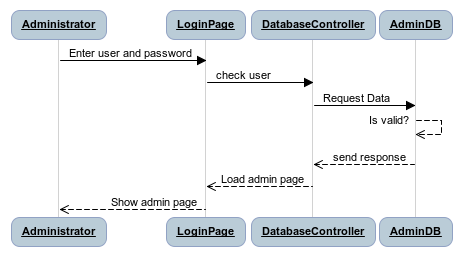
\includegraphics[width=10.1cm]{pics/loginse.png}
  \end{center}
\caption{Administrator's Login.}
\end{figure}
\newpage
\subsection{Upload Experiments}
%\vskip 1cm
\begin{figure}[!hp]
  \begin{center}
   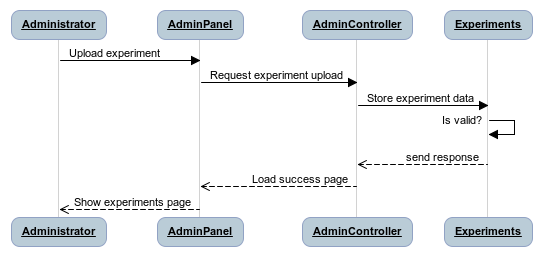
\includegraphics[width=11.3cm]{pics/upload.png}
  \end{center}
\caption{Upload experiment.}
\end{figure}


\subsection{Download Experiments}
%\vskip 1cm
\begin{figure}[!hp]
  \begin{center}
   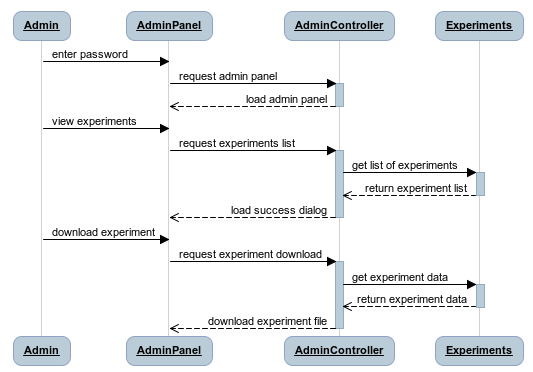
\includegraphics[width=11.6cm]{pics/download_experiments.png}
  \end{center}
\caption{Download Experiment.}
\end{figure}

\newpage

\vskip 1cm
\subsection{View Experiments}
\vskip 1cm
\begin{figure}[!hp]
  \begin{center}
   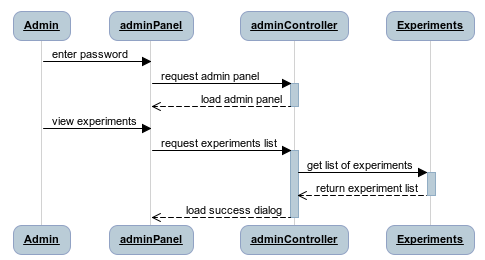
\includegraphics[width=10.8cm]{pics/view_experiments.png}
  \end{center}
\caption{View Experiments.}
\end{figure}

%\vskip 1.5cm
% The diagram shows the interation between the \emph{participant} with the \emph{system}, in order to take a \emph{survey}.

\newpage

\section{Activity Diagrams}
\subsection {Survey creation}
\begin{figure}[h!]
  \begin{center}
   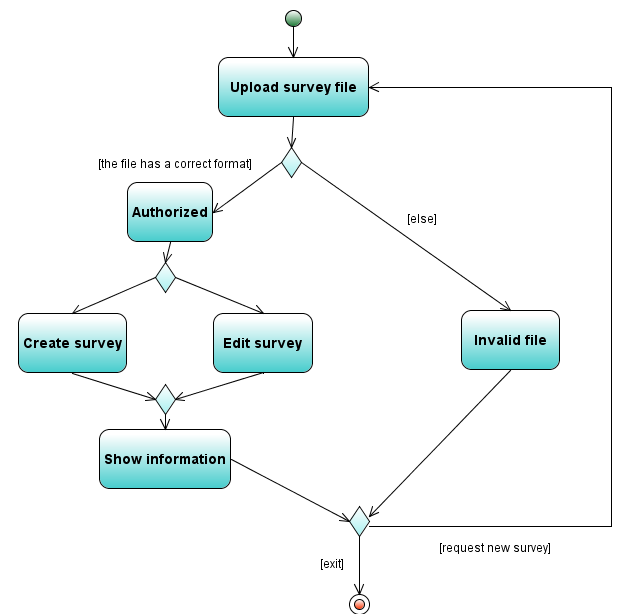
\includegraphics[width=13.5cm]{pics/Activity.png}
  \end{center}
\caption{Activity Diagram for survey creation.}
\end{figure}
This is a graphical representation of workflows of the activity of survey creation. It shows the steps needed to be followed in order to upload a new survey (or as we call it \emph{experiment}). The administrator selects a file to upload. They system will check the validity of the file format, if correct the user can either make final changes or create it. If the format is incorrect, the system will show the error and request a new file.
\newpage
\subsection{Survey Management}
\begin{figure}[!hp]
  \begin{center}
   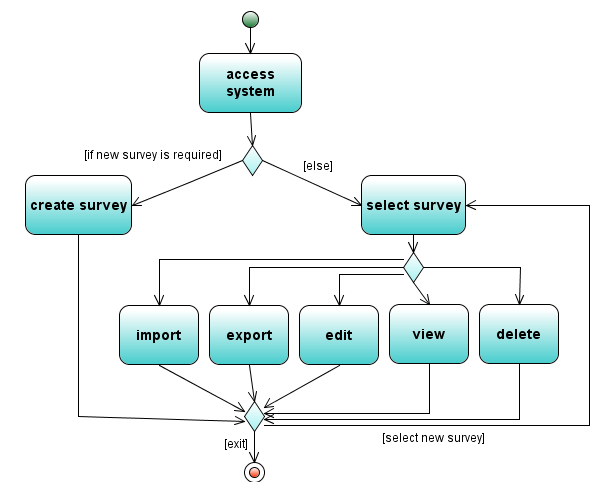
\includegraphics[width=13.76cm]{pics/Activity2.png}
  \end{center}
\caption{Activity Diagram for survey management.}
\end{figure}
\vskip 1cm
This activity diagram represents operational step-by-step work-flows of the survey management. The main options that the system will allow the administrator to perform related to experiments is their creation or edition. In order to perform basic operations such as {\it import, export} or {\it delete}, you need to select the survey to which you are going to apply the operations.

\pagebreak
\pagebreak
\section{Use Case Diagrams}
\vskip 1cm
\begin{figure}[h!]
  \begin{center}
   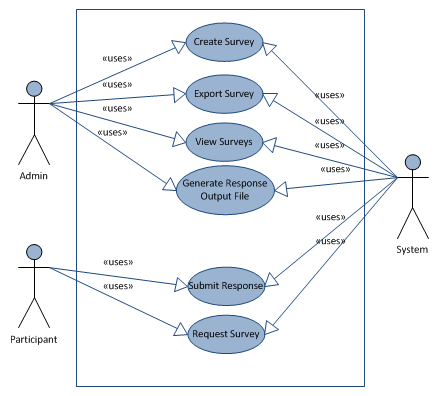
\includegraphics[width=12.2cm]{pics/usecase.png}
  \end{center}
\caption{Main Use Case Diagram.}
\end{figure}
\vskip 1cm
This use case shows the main basic functions of our system. There are to main actors that will interact with the system, the \emph{administrator} and the \emph{paticipant}. Each of them will be able to perform some tasks, as specified by the previous figure.

\newpage
\vskip 1cm
\begin{figure}[h!]
  \begin{center}
   \includegraphics[width=15cm]{pics/manageSurveys.png}
  \end{center}
\caption{Survey Management.}
\end{figure}
\vskip 1cm
This use case represents the basic interaction of the administrator with the Surveys. The surveys is the main focus of our application, that is why the Administrator has capabilities for total interaction with them.


\chapter{ Restrictions, Limitations, and Contraints}

\section{ Description For Experiment Component}
An experiment will consist in a set of surveys. Each survey should be able to contain three types of inputs:
\begin{description}
\item [Text box.] It will consists of 0 or more integers.
\item [Radio box.] Containing one number. It is inclusive.
\item  [Yes/No radio box.] Allowing a two choice answer.
\end{description}
The system will support infinite surveys and experiments.

\section{ Description For User Component}

The user or participant shall be able to perform the following actions:
\begin{itemize}
	\item Request Survey by URL \\ Correct survey automatically assigned to user based off URL.
	\item Submit Survey Response
\end{itemize}
\section{  Description For Administrator Component}

Although our design will allow the possibility of future additions of administers easily, initially we will only have one. The administrator shall be able to do the following actions:
\begin{itemize}
	\item Create Survey \\ transfer a new xlsx file via ftp to an input folder
	\item Edit Survey \\ overrides the existing xlsx file
	\item View Survey \\ downloads the xlsx file from the server
	\item Download Results 
\end{itemize}

\section{Description for the Output File}
The exported results will be in {\bf csv} format. The mush contain the following restrictions:
\begin {itemize}
\item Additional column for survey title.
 \item Do not have to support excel.
\end{itemize}


\chapter{ User Interface Design}

\section{  Description Of The User Interface}

The main features that the software will present are:
\begin{itemize}
\item {\it Sets of surveys}, allowing the user to automatically loop through them.
\item {\it Pseudo-Randomization} of the order of the surveys.
\item {\it Result file}. This file will contain these main fields: Subject ID, survey number, code and responses.
\end{itemize}

\subsubsection { Appearance Of Surveys}
\begin{itemize} 
	\item  the appearance of the sentences on the web form (font, size, color, spacing, location, etc) needs to be customizable through CSS/HTML tags
	\item the web form needs to accept a couple of different response types (radio buttons, text boxes, etc)
	\item Left/Center/Right justifiable
	\item autocomplete off
	\item css template file option
	\item sentences per page
\end{itemize}

\subsection{ Screen Images }
\vskip 0.8cm
\subsubsection{Login Screen}
\begin{figure}[h!!]
  \begin{center}
   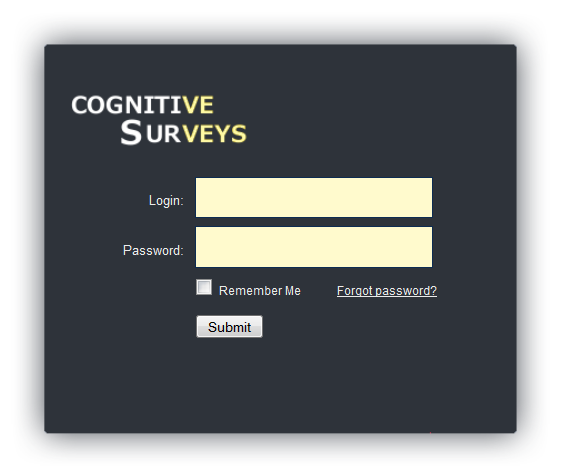
\includegraphics[width=10.7cm]{pics/login.png}
  \end{center}
\caption{Login Screen.}
\end{figure}
\vskip  1.4cm
This is the first page that appears to the administrator while the application. It will request an user name and the password. If the input is correct (matches with the records in the database), the main administration panel will show up.

\newpage
\subsubsection{Admin Screen}
\begin{figure}[hp!!]
  \begin{center}
   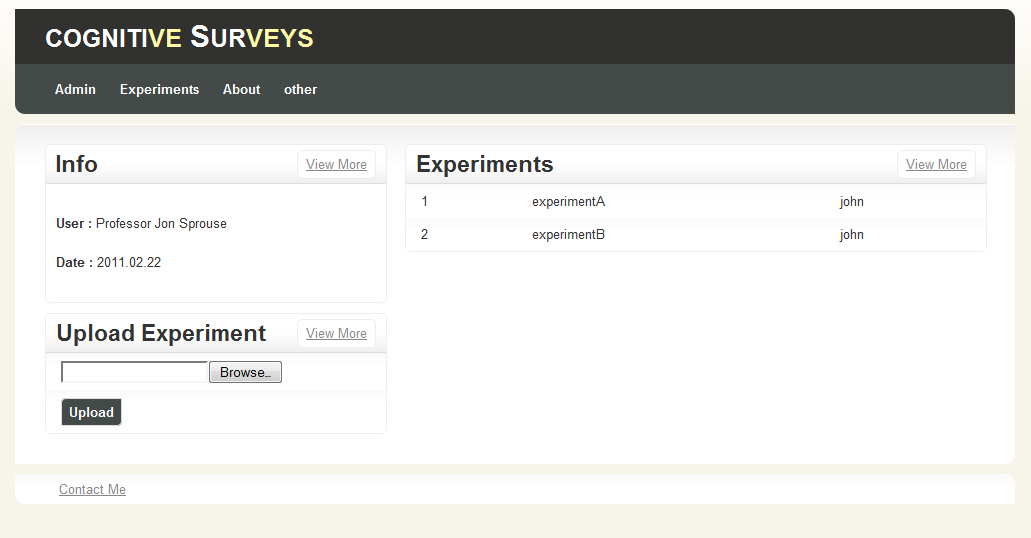
\includegraphics[width=14cm]{pics/adminPage.png}
  \end{center}
\caption{Adminisrator Screen.}
\end{figure}
Main page where the administrator can perform the main operations of survey management.
\subsubsection{List of Experiments Screen}
\begin{figure}[hp!!]
  \begin{center}
   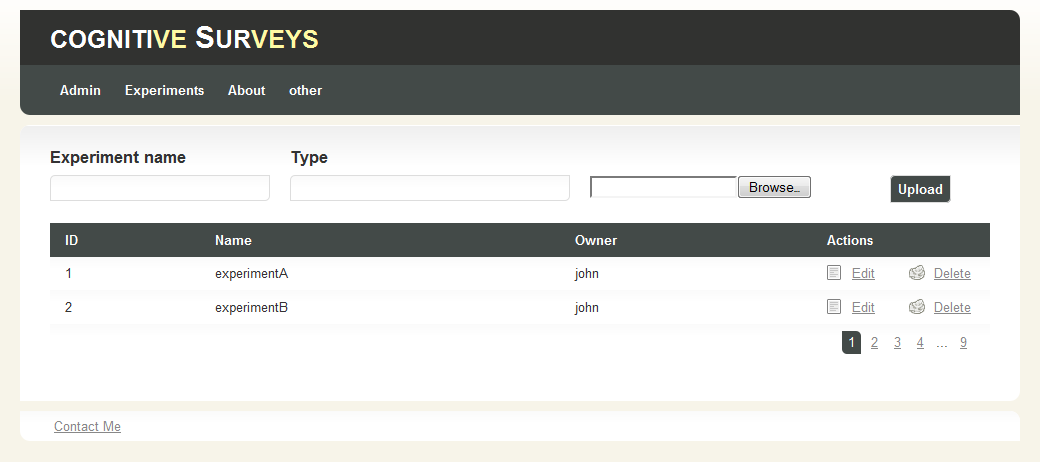
\includegraphics[width=14cm]{pics/experiments.png}
  \end{center}
\caption{Screen showing list of experiments.}
\end{figure}

\newpage
\subsubsection{Survey Screen}
\begin{figure}[h!!]
  \begin{center}
   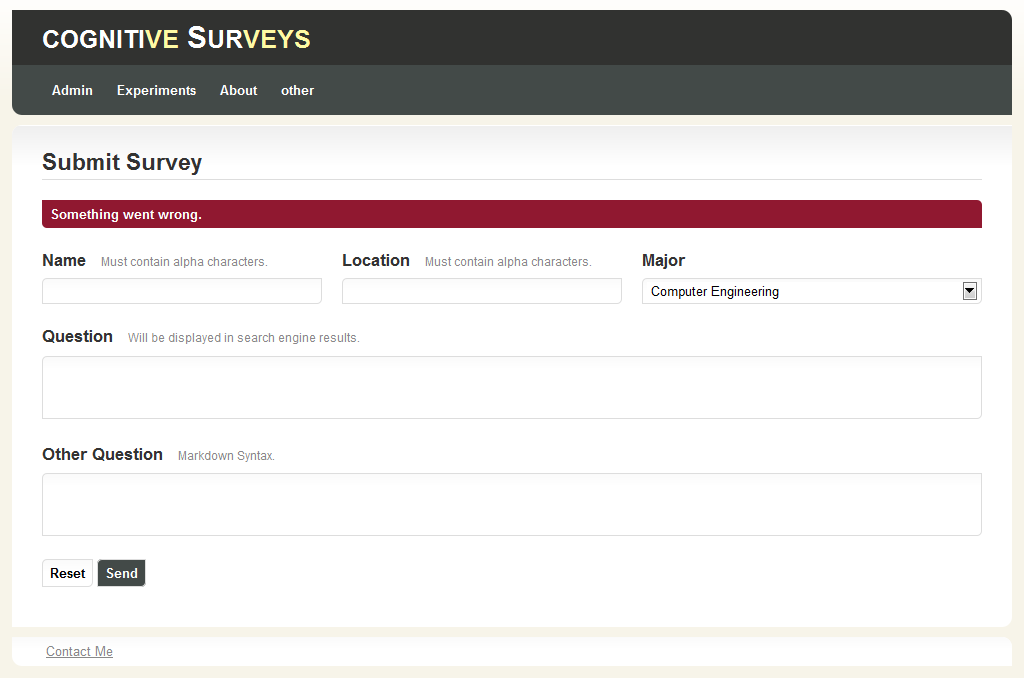
\includegraphics[width=14cm]{pics/survey.png}
  \end{center}
\caption{Survey Screen.}

\end{figure}
\vskip 1cm
Sample screen of how a survey might look like. The red high-lighted text shows when the user sent the survey but he did not fill all fields correctly.



\end{document}
